
\documentclass{beamer}

% for themes, etc.
\mode<presentation>
{ \usetheme{Torino} }
%{ \usetheme{boxes} }

\usepackage{times}  % fonts are up to you
\usepackage{graphicx}

% these will be used later in the title page
\title{CHPC WLCG Tier2 Facility}
\author{Sean Murray \\
    CHPCs \\
    CSIR 
}
\date{July 7, 2016}

% note: do NOT include a \maketitle line; also note that this title
% material goes BEFORE the \begin{document}

% have this if you'd like a recurring outline
\AtBeginSection[]  % "Beamer, do the following at the start of every section"
{
\begin{frame}<beamer> 
\frametitle{Outline} % make a frame titled "Outline"
\tableofcontents[currentsection]  % show TOC and highlight current section
\end{frame}
}

\begin{document}

% this prints title, author etc. info from above
\begin{frame}
\titlepage
\end{frame}

\section{WLCG}

\begin{frame}
\frametitle{ALICE}

(Illustrating {\sc beamer}'s $\backslash$pause command.)
\vskip 0.5in

A couple of years ago, a fifth-grade teacher asked me to explain to her
the reasoning behind the ``invert and multiply'' rule for dividing
fractions, e.g.
\pause  % makes overlay

$$
\frac{4}{5} \div \frac{2}{3} = \frac{4}{5} \times \frac{3}{2}
$$

\pause

Let's try to find answers understandable by fifth graders (at least the
more patient ones).

\end{frame}

\begin{frame}
\frametitle{ALICE MUON Arm}

Here let's just use intuition, understandable by fifth graders.

\pause

If we give 1/3 of a cookie to each person, how many people can we
feed with 1 cookie?  

\pause

Obviously, the answer is 3.

So we've derived the ``invert and multiply'' rule in a special case:

$$
1 \div \frac{1}{3} = 3
$$

\end{frame}

\begin{frame}
\frametitle{Detector Structure}

But what if we give 2/3 of a cookie, not 1/3, to each person?  

We're giving 2$\times$ as much per person. 

So we can feed only 1/2 as many people. 

So we feed  $\frac{1}{2} \times 3 = \frac{3}{2}$.\footnote{One person
gets only a half share.}

So we've derived the ``invert and multiply'' rule in another case:

$$
1 \div \frac{2}{3} = \frac{3}{2}
$$

\end{frame}

\begin{frame}
\frametitle{Detector Structure 2}

Now, suppose we have only 4/5 of a cookie.

Then we can feed only 4/5 as many people, i.e.

$$
\frac{4}{5} \times \frac{3}{2} ~ people
$$

\pause 

So we've derived the ``invert and multiply'' rule in the general case:

$$
\frac{4}{5} \div \frac{2}{3} = \frac{4}{5} \times \frac{3}{2}
$$ 

\end{frame}

\section{Three pillars}

\begin{frame}
\frametitle{Current MUON Software}

(Illustrating {\sc beamer}'s $\backslash$uncover command.)
\vskip 0.5in

\begin{theorem}
The angles in a triangle sum to $180^{\circ}$.
\end{theorem}

\pause

Plan:  Extend AC past C to D.  Draw CE parallel to AB.

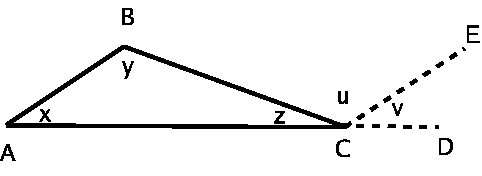
\includegraphics[width = 2.0in]{BeamerTriangle.jpg}  

\end{frame}

\begin{frame}

\begin{proof}

\begin{tabular}{ll}
% uncover makes advanced overlay
\uncover<1->{1. u = y} & \uncover<2->{Alternate angles of a
transveral.} \\ 
\uncover<3->{2. v = x} & \uncover<4->{Consecutive interior angles of a
transveral} \\ 
\uncover<5->{3. z+u+v = $180^{\circ}$} & \uncover<6->{ACD is a straight
line.} \\ 
\uncover<7->{4. z+y+x = $180^{\circ}$} & \uncover<8->{Substitution
from Steps 1 and 2.} \\
\end{tabular}

\end{proof}

\end{frame}

\section{Tier1}

\begin{frame}
\frametitle{What is a cluster finder} 

\begin{itemize}

\item This tour just scratches the surface.  
\pause

\item {\sc beamer} has enough features to fill a 210-page user manual!  
\pause

\item Advanced example:
\url{http://latex-beamer.sourceforge.net/beamerexample1.pdf}.

\end{itemize}

\end{frame}

\end{document}

